
\section{Feed-Forward (Prealimentación)} % G_h y G_w


El control retroalimentado (Feedback) tradicional posee una limitación inherente: requiere que exista un error en la variable de proceso para poder actuar. Para compensar esta inercia, se implementa una arquitectura de prealimentación o \textit{Feedforward} (FF), la cual mide las variables de entrada al sistema e inyecta una acción de control antes de que la variable controlada se vea afectada.

\begin{figure}[ht]
  \begin{center}
    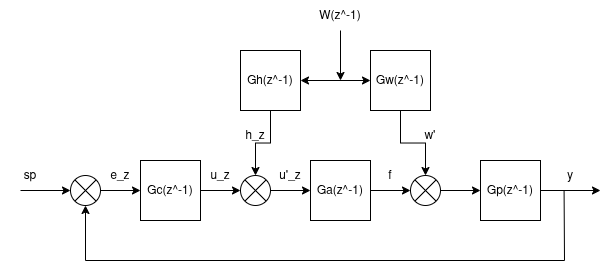
\includegraphics[width=0.95\textwidth]{figures/ff.png}
  \end{center}
  \caption{}\label{fig:ff}
\end{figure}
\subsubsection{Obtención Matemática: Compensación de Perturbaciones}

Considérese un sistema donde la salida $y(z^{-1})$ se ve afectada tanto por la acción de control $u_z$ a través de la planta $G_p(z^{-1})$ y el actuador $G_a(z^{-1})$, como por una perturbación medible $W(z^{-1})$ a través de su propia dinámica $G_w(z^{-1})$. La ecuación en el dominio $Z$ es:
\[
  Y(z^{-1}) =G_p(z^{-1}) \left[ (u_{z}(z^{-1}) + h_{h}(z^{-1})) G_a(z^{-1}) + W(z^{-1}) G_w(z^{-1}) \right]
\]
\[
Y(z^{-1}) = G_p(z^{-1})\left[ (u_{z}(z^{-1}) + W(z^{-1})G_h(z^{-1})) G_a(z^{-1})  + W(z^{-1}) G_w(z^{-1})\right]
\]
\[ 
  Y(z^{-1}) = G_p(z^{-1})\left[u_z(z^{-1})G_a(z^{-1})G_p(z^{-1}) + W(z^{-1})G_h(z^{-1})G_a(z^{-1}) + W(z^{-1})G_w(z^{-1})\right]  
\]

\begin{equation}
  Y(z^{-1}) = \underbrace{(Sp - Pv)G_c(z^{-1})G_a(z^{-1})G_p(z^{-1})}_{\text{PID}} + \underbrace{W(z^{-1})G_h(z^{-1})G_a(z^{-1})G_p(z^{-1}) + W(z^{-1})G_w(z^{-1})G_p(z^{-1})}_{\text{Feed-Forward}}  
  \label{eq:ff2}
\end{equation}

\clearpage


El objetivo del compensador de perturbaciones es lograr una invariancia perfecta, es decir, que el efecto de $W(z^{-1})$ sobre $Y(z^{-1})$ sea nulo ($Y(z^{-1}) = 0$ asumiendo $u_{z}=0$). Igualando a cero la contribución de la perturbación, se despeja la acción de control anticipatoria:
\[
  0 = W(z^{-1})G_h(z^{-1})G_a(z^{-1})G_p(z^{-1}) + W(z^{-1})G_w(z^{-1})G_p(z^{-1}) 
\]

\begin{equation}
  G_h(z^{-1}) = -\frac{G_w(z^{-1})}{G_a(z^{-1})} 
  \label{eq:G_w}
\end{equation}
Definiendo el bloque compensador como $
  G_h(z^{-1}) = -\frac{G_w(z^{-1})}{G_a(z^{-1})} 
$, se logra la cancelación algebraica de la perturbación entrante.

\subsubsection{Obtención Matemática: Compensación Estática de No Linealidad}
Si bien con el esquema anterior se neutraliza el efecto de la perturbación sobre el sistema, aún se debe considerar su naturaleza no lineal dada por las descargas por gravedad en cada estanque.

Se puede aplicar un raciocinio idéntico para mejorar el seguimiento de la referencia ($SP$). En lugar de esperar a que el integrador del PID acumule la energía necesaria para alcanzar el nivel deseado, se puede pre-calcular el esfuerzo de control exacto (alimentando el sp al feeedforward), o corregir la no linealidad en cada valor de nivel (alimentar el pv al feedforward). 

Es fundamental destacar que \textbf{no se invierte la dinámica completa de la planta} (lo cual requeriría la derivada de la referencia y generaría un esfuerzo de control irrealizable). En su lugar, el Feedforward en este caso invierte únicamente la \textbf{ganancia estática} del proceso. 

En sistemas con dinámicas complejas como el de los 4 estanques, esta ganancia estática contiene la principal no linealidad del sistema (la fuga de Torricelli). Al inyectar una señal de prealimentación que es la inversa exacta de esta no linealidad ($G_{sp} = G_{estatico}^{-1}$), se logran dos objetivos simultáneos:

\begin{enumerate}
    \item Proporcionar al actuador la energía base requerida para sostener el nivel del Setpoint deseado en estado estacionario.
    \item Linealizar el sistema desde la perspectiva del lazo cerrado, permitiendo que el controlador PID solo deba encargarse de corregir las inercias transitorias dinámicas y los pequeños errores de modelación.
\end{enumerate}


\begin{figure}[ht]
  \begin{center}
    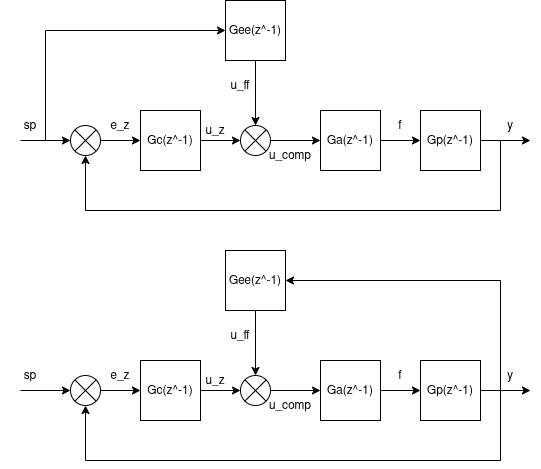
\includegraphics[width=0.8\textwidth]{figures/ff_sp.png}
  \end{center}
  \caption{Feedforward de compensación (PV y SP)}
  \label{fig:ffsp}
\end{figure}

Ignorando la perturbación y la acción del controlador temporalmente, se busca que la salida alcance la referencia ($Y(z^{-1}) = SP(z^{-1})$) utilizando exclusivamente una acción precalculada $U_{FF\_SP}(z^{-1})$:

\begin{align}
    SP(z^{-1}) &= U_{FF\_SP}(z^{-1}) G_a(z^{-1}) G_p(z^{-1}) \\
    U_{FF\_SP}(z^{-1}) &= SP(z^{-1}) \frac{1}{G_a(z^{-1}) G_p(z^{-1})}
\end{align}

Definiendo este segundo bloque como $G_{sp}(z^{-1}) = \frac{1}{G_a(z^{-1}) G_p(z^{-1})}$, se establece un control de \textit{2 Grados de Libertad}, donde el Feedforward proporciona el esfuerzo base y el PID se encarga únicamente de corregir errores dinámicos y no linealidades residuales no modeladas.
\clearpage
\subsubsection{SP vs PV}

Para tomar una decisión de diseño justificada, el ingeniero debe balancear la precisión matemática contra la robustez física de los actuadores y la facilidad de sintonía figura \ref{fig:ffsp}.

\vspace{3mm}
\noindent\textbf{Enfoque A: Linealización por Realimentación (Usar PV)}
\begin{itemize}
    \item[\textcolor{green!60!black}{\textbf{+}}] \textbf{Linealidad Perfecta:} La no linealidad (parábola) se cancela en absolutamente todo momento, sin importar si el estanque se está llenando, vaciando o está en equilibrio.
    \item[\textcolor{green!60!black}{\textbf{+}}] \textbf{Independencia del Punto de Operación:} Un solo conjunto de ganancias PID funcionará exactamente igual de bien con el estanque a 10 cm que a 40 cm.
    \item[\textcolor{red}{\textbf{--}}] \textbf{Sensibilidad al Ruido (Inyección de Oleaje):} Este es su mayor defecto físico. El sensor de nivel real ($LIT$) siempre tiene ruido debido al oleaje del agua y turbulencias. Al meter la $PV$ en la ecuación, ese ruido entra directo al cálculo de la raíz cuadrada y se envía como órdenes erráticas de voltaje al variador de frecuencia, desgastando mecánicamente la bomba (\textit{chattering}).
    \item[\textcolor{red}{\textbf{--}}] \textbf{Sintonía Compleja:} Al cancelar la fuga de agua matemáticamente, el estanque se comporta como un integrador puro. Los sistemas integradores son inherentemente más inestables y difíciles de sintonizar (suelen requerir acción derivativa cuidadosa o un PI muy conservador para no oscilar).
\end{itemize}

\vspace{3mm}
\noindent\textbf{Enfoque B: Control de 2 Grados de Libertad (Usar SP)}
\begin{itemize}
    \item[\textcolor{green!60!black}{\textbf{+}}] \textbf{Inmunidad al Ruido Analógico:} El Setpoint ($SP$) es una variable matemática pura y limpia generada por el software. Al usarla en el cálculo, la señal base enviada a la bomba es perfectamente estable, prolongando la vida útil del actuador.
    \item[\textcolor{green!60!black}{\textbf{+}}] \textbf{Sintonía Dócil (Autorregulación):} Como no se cancela la dinámica natural del estanque, el sistema sigue siendo autorregulado (un sistema de primer orden tradicional). Es extremadamente fácil y seguro sintonizar un controlador PI para este tipo de plantas.
    \item[\textcolor{red}{\textbf{--}}] \textbf{Error en el Transitorio:} La compensación de la no linealidad solo es matemáticamente perfecta cuando el sistema alcanza el estado estacionario ($PV = SP$). Durante el llenado o vaciado, el PID debe trabajar un poco más para compensar la diferencia.
    \item[\textcolor{red}{\textbf{--}}] \textbf{Golpe al Actuador (Derivada del Escalón):} Si el operador introduce un cambio de $SP$ muy grande, la ecuación calculará una demanda de energía instantánea masiva. \textbf{Solución obligatoria:} Se debe implementar un filtro de Setpoint (una rampa de aceleración en la HMI o en el PLC) para suavizar la transición del operador.
\end{itemize}

\subsubsection{Aplicación a las Ecuaciones de Diferencias de la Planta}
Para aplicar esta teoría lineal a los estanques no lineales, evaluamos la derivada del balance de masas en estado estacionario ($\frac{dh}{dt} = 0$). Tomando como ejemplo el Estanque 1 (que sufre la perturbación de caudal del Estanque 3), la Ecuación \ref{eq:edo_h1} se iguala a cero.

Forzando que en estado estacionario el nivel alcance el Setpoint ($h_1 = SP_1$), y despejando la acción de control de la bomba ($u_1$), obtenemos la ley de control Feedforward pura (sin considerar aún la acción del PID):
\begin{align}
    0 &= -a_1 \sqrt{2g \cdot SP_1} + a_3 \sqrt{2g \cdot h_3} + \gamma_1 k_1 u_1 \nonumber \\
    \gamma_1 k_1 u_1 &= a_1 \sqrt{2g \cdot SP_1} - a_3 \sqrt{2g \cdot h_3} \nonumber \\
    u_1 &= \underbrace{\frac{a_1 \sqrt{2g \cdot SP_1}}{\gamma_1 k_1}}_{\text{Término } G_h \text{ (Referencia)}} - \underbrace{\frac{a_3 \sqrt{2g \cdot h_3}}{\gamma_1 k_1}}_{\text{Término } C_w \text{ (Perturbación)}}
\end{align}

Al integrar esto con el algoritmo digital dentro del PLC, la señal de control total en el instante discreto $[k]$ resulta en la suma de prealimentación y el control retroalimentado:
\begin{equation}
    u_{total}[k] = u_{PID}[k] + \frac{a_1 \sqrt{2g \cdot SP_1[k]}}{\gamma_1 k_1} - \frac{a_3 \sqrt{2g \cdot h_3[k]}}{\gamma_1 k_1}
\end{equation}
